\documentclass[../Article_Sensitivity_Analsysis.tex]{subfiles}
\graphicspath{{\subfix{../Figures/}}}
\begin{document}
	
	To identify the global solution for Equations \ref{EQ:Formulation_2}, the optimization problem is solved multiple times, each run starting from a random initial solution sampled from a uniform distribution. Figure \ref{fig:scatter} compares the initial and final cost function values across multiple optimization runs for all pressure cases. The solution with the lowest cost function value is considered the global solution for each case.
	
	\begin{figure}[h!]
		\centering
		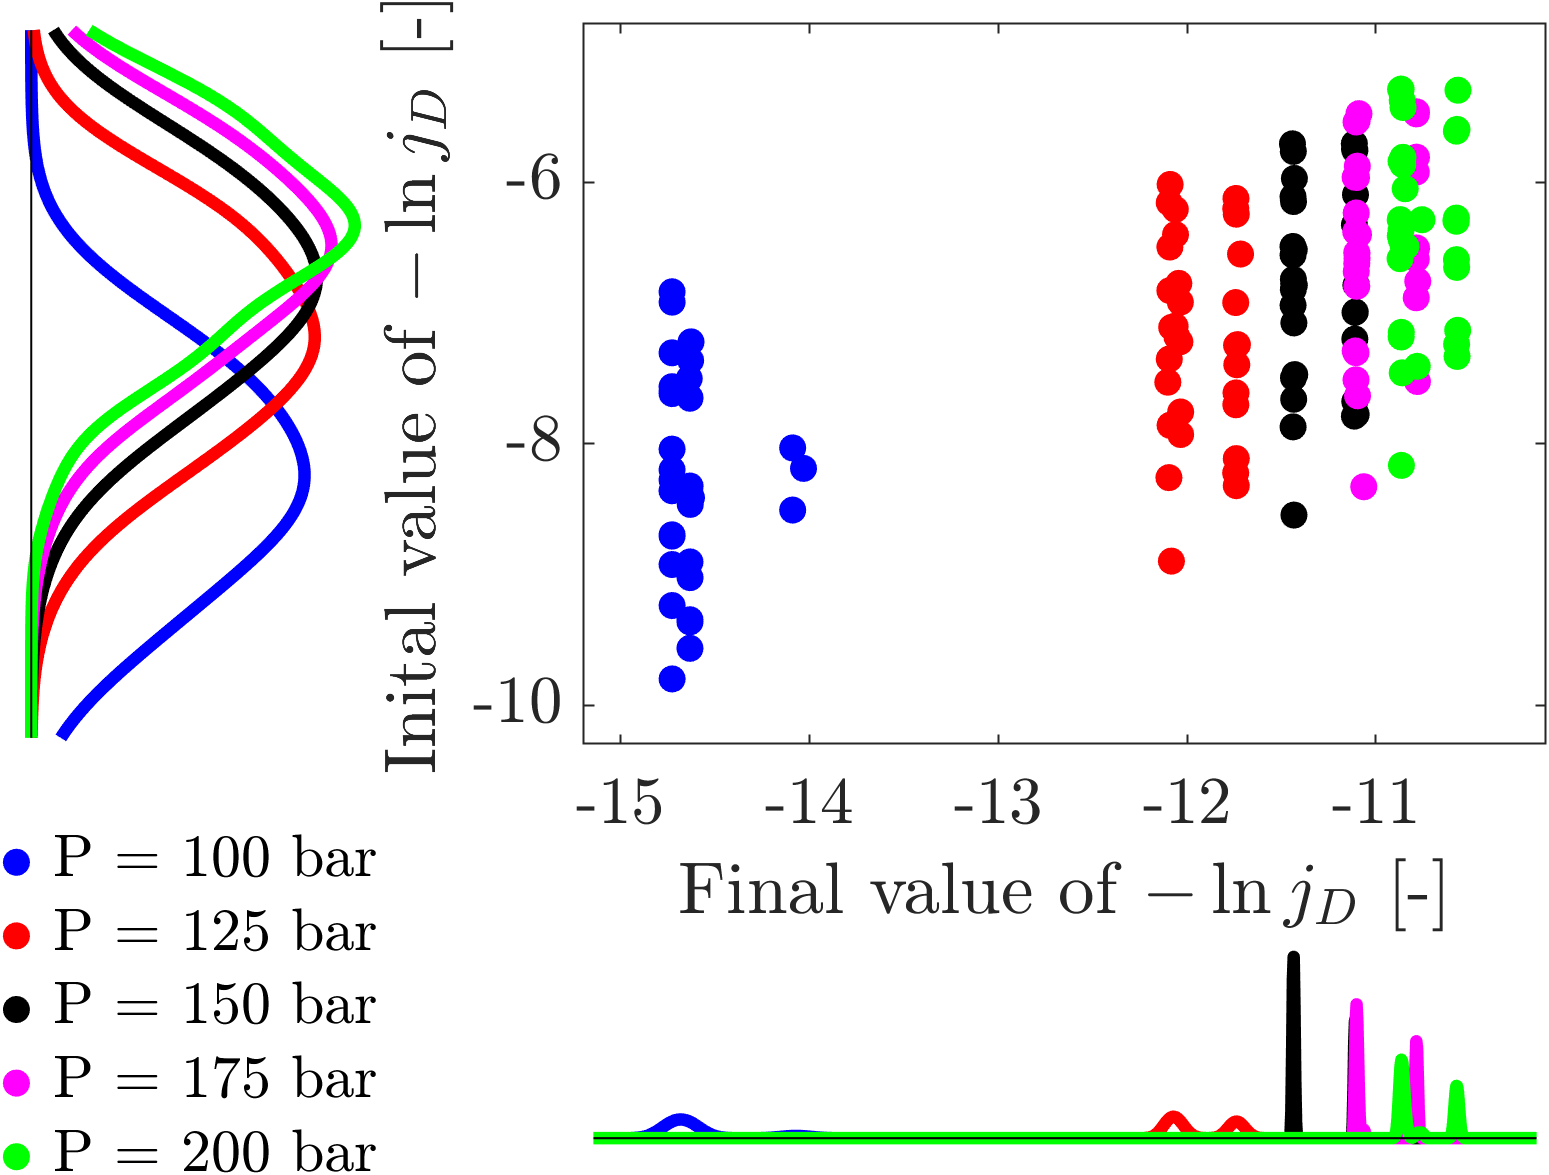
\includegraphics[width=0.90\columnwidth]{Figures/Results/scatter.png}	
		\caption{Initial vs final values of the cost function}
		\label{fig:scatter}
	\end{figure}
	
	By analyzing locations of the clusters in Figure \ref{fig:scatter}, it can be concluded that experiments conducted near the critical point provide more information regarding the correlation than those conducted farther from it. For each pressure case, the solutions with the lowest value of the objective function are further analysed. The closer the pressure is to the critical point, the larger the deviations in the physical properties of $CO_2$ caused by changes in the controls, leading to greater variation in the Reynolds number, and consequently to more informative experiments. 
	
	As presented in Figure \ref{fig:profiles_F}, all mass flow rate profiles initially stay at a minimum value, persisting for 100 to 150 minutes, depending on the pressure. Subsequently, a step-like increase in mass flow rate is observed, with the onset occurring earlier at higher pressures. Between 250 and 300 min, the mass flow rate stabilizes at value of the upper bound.
	
	\begin{figure}[t!]
		\centering
		\begin{subfigure}[t]{\columnwidth}
			\centering
			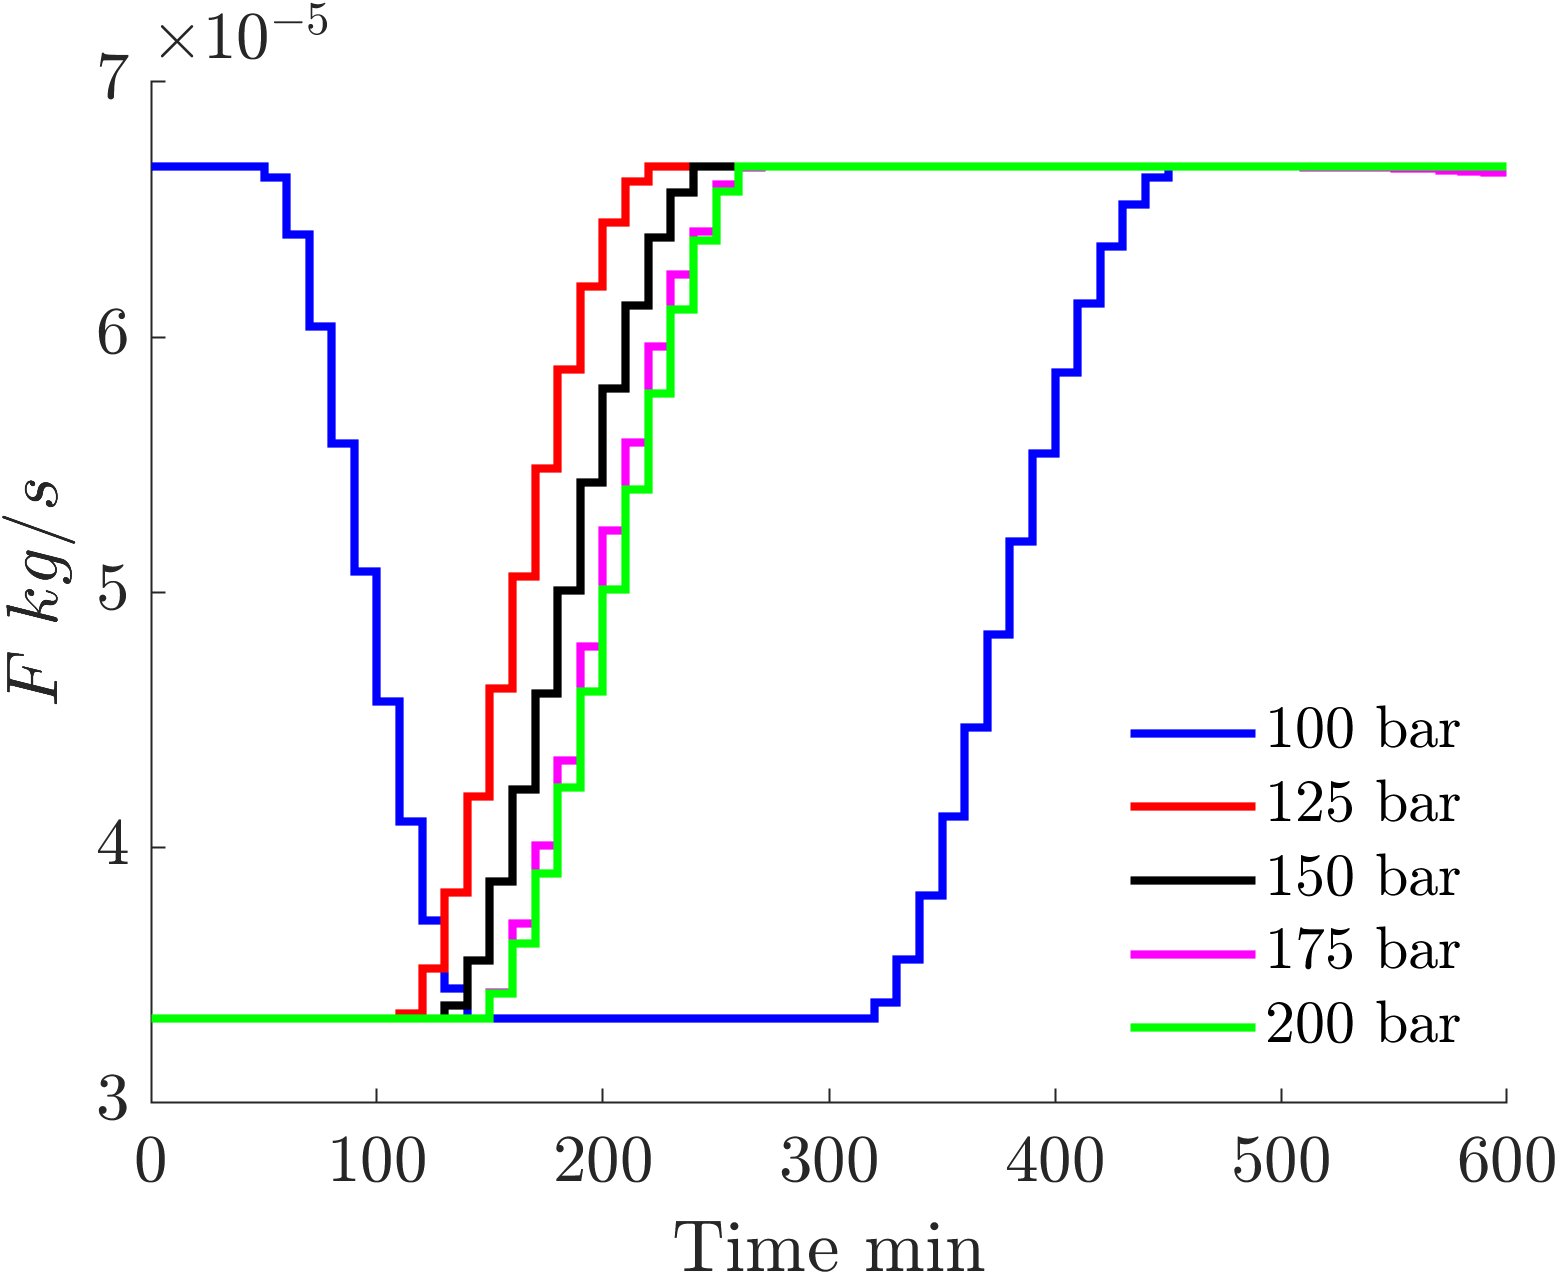
\includegraphics[width=0.90\columnwidth]{Figures/Results/Profile_F.png}	
			\caption{Optimal mass flow rate profiles}
			\label{fig:profiles_F}
		\end{subfigure}%
		\par\bigskip % force a bit of vertical whitespace
		\begin{subfigure}[t]{\columnwidth}
			\centering
			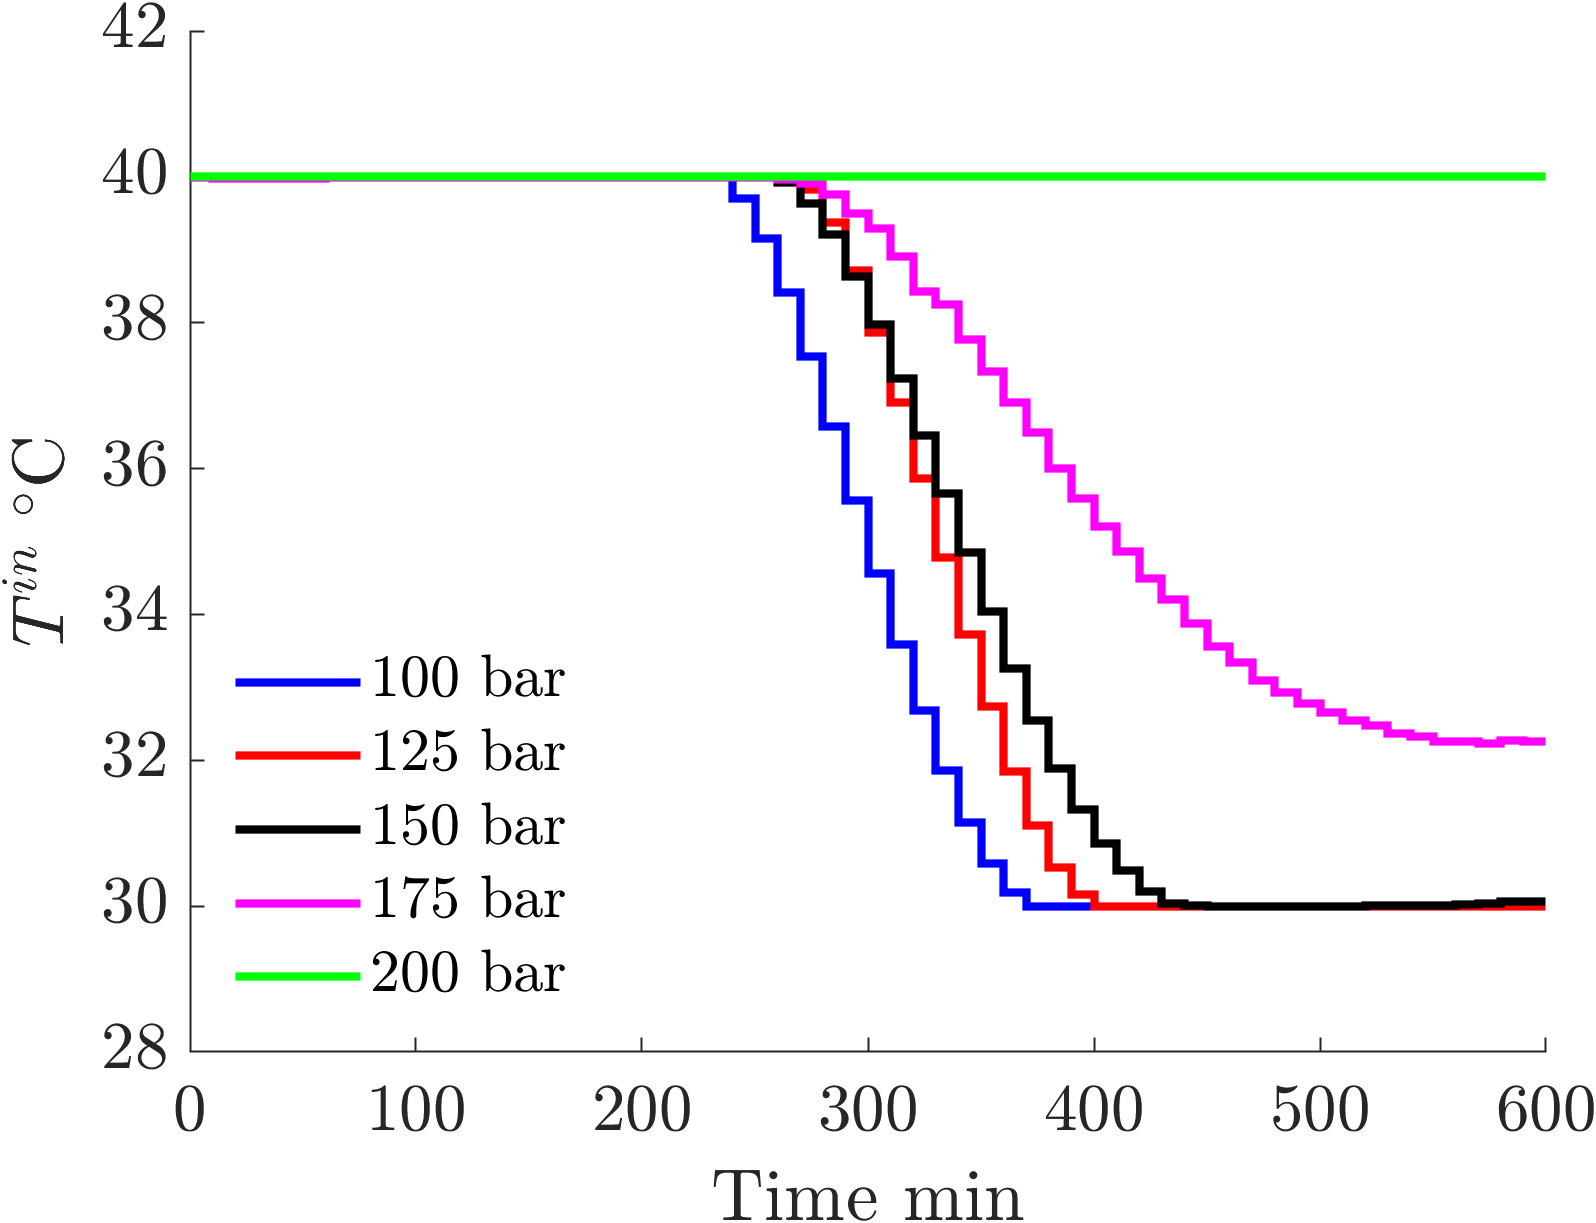
\includegraphics[width=0.90\columnwidth]{Figures/Results/Profile_T.png}	
			\caption{Optimal inlet temperature profile}
			\label{fig:profiles_T}
		\end{subfigure}
		\par\bigskip % force a bit of vertical whitespace
		\begin{subfigure}[t]{\columnwidth}
			\centering
			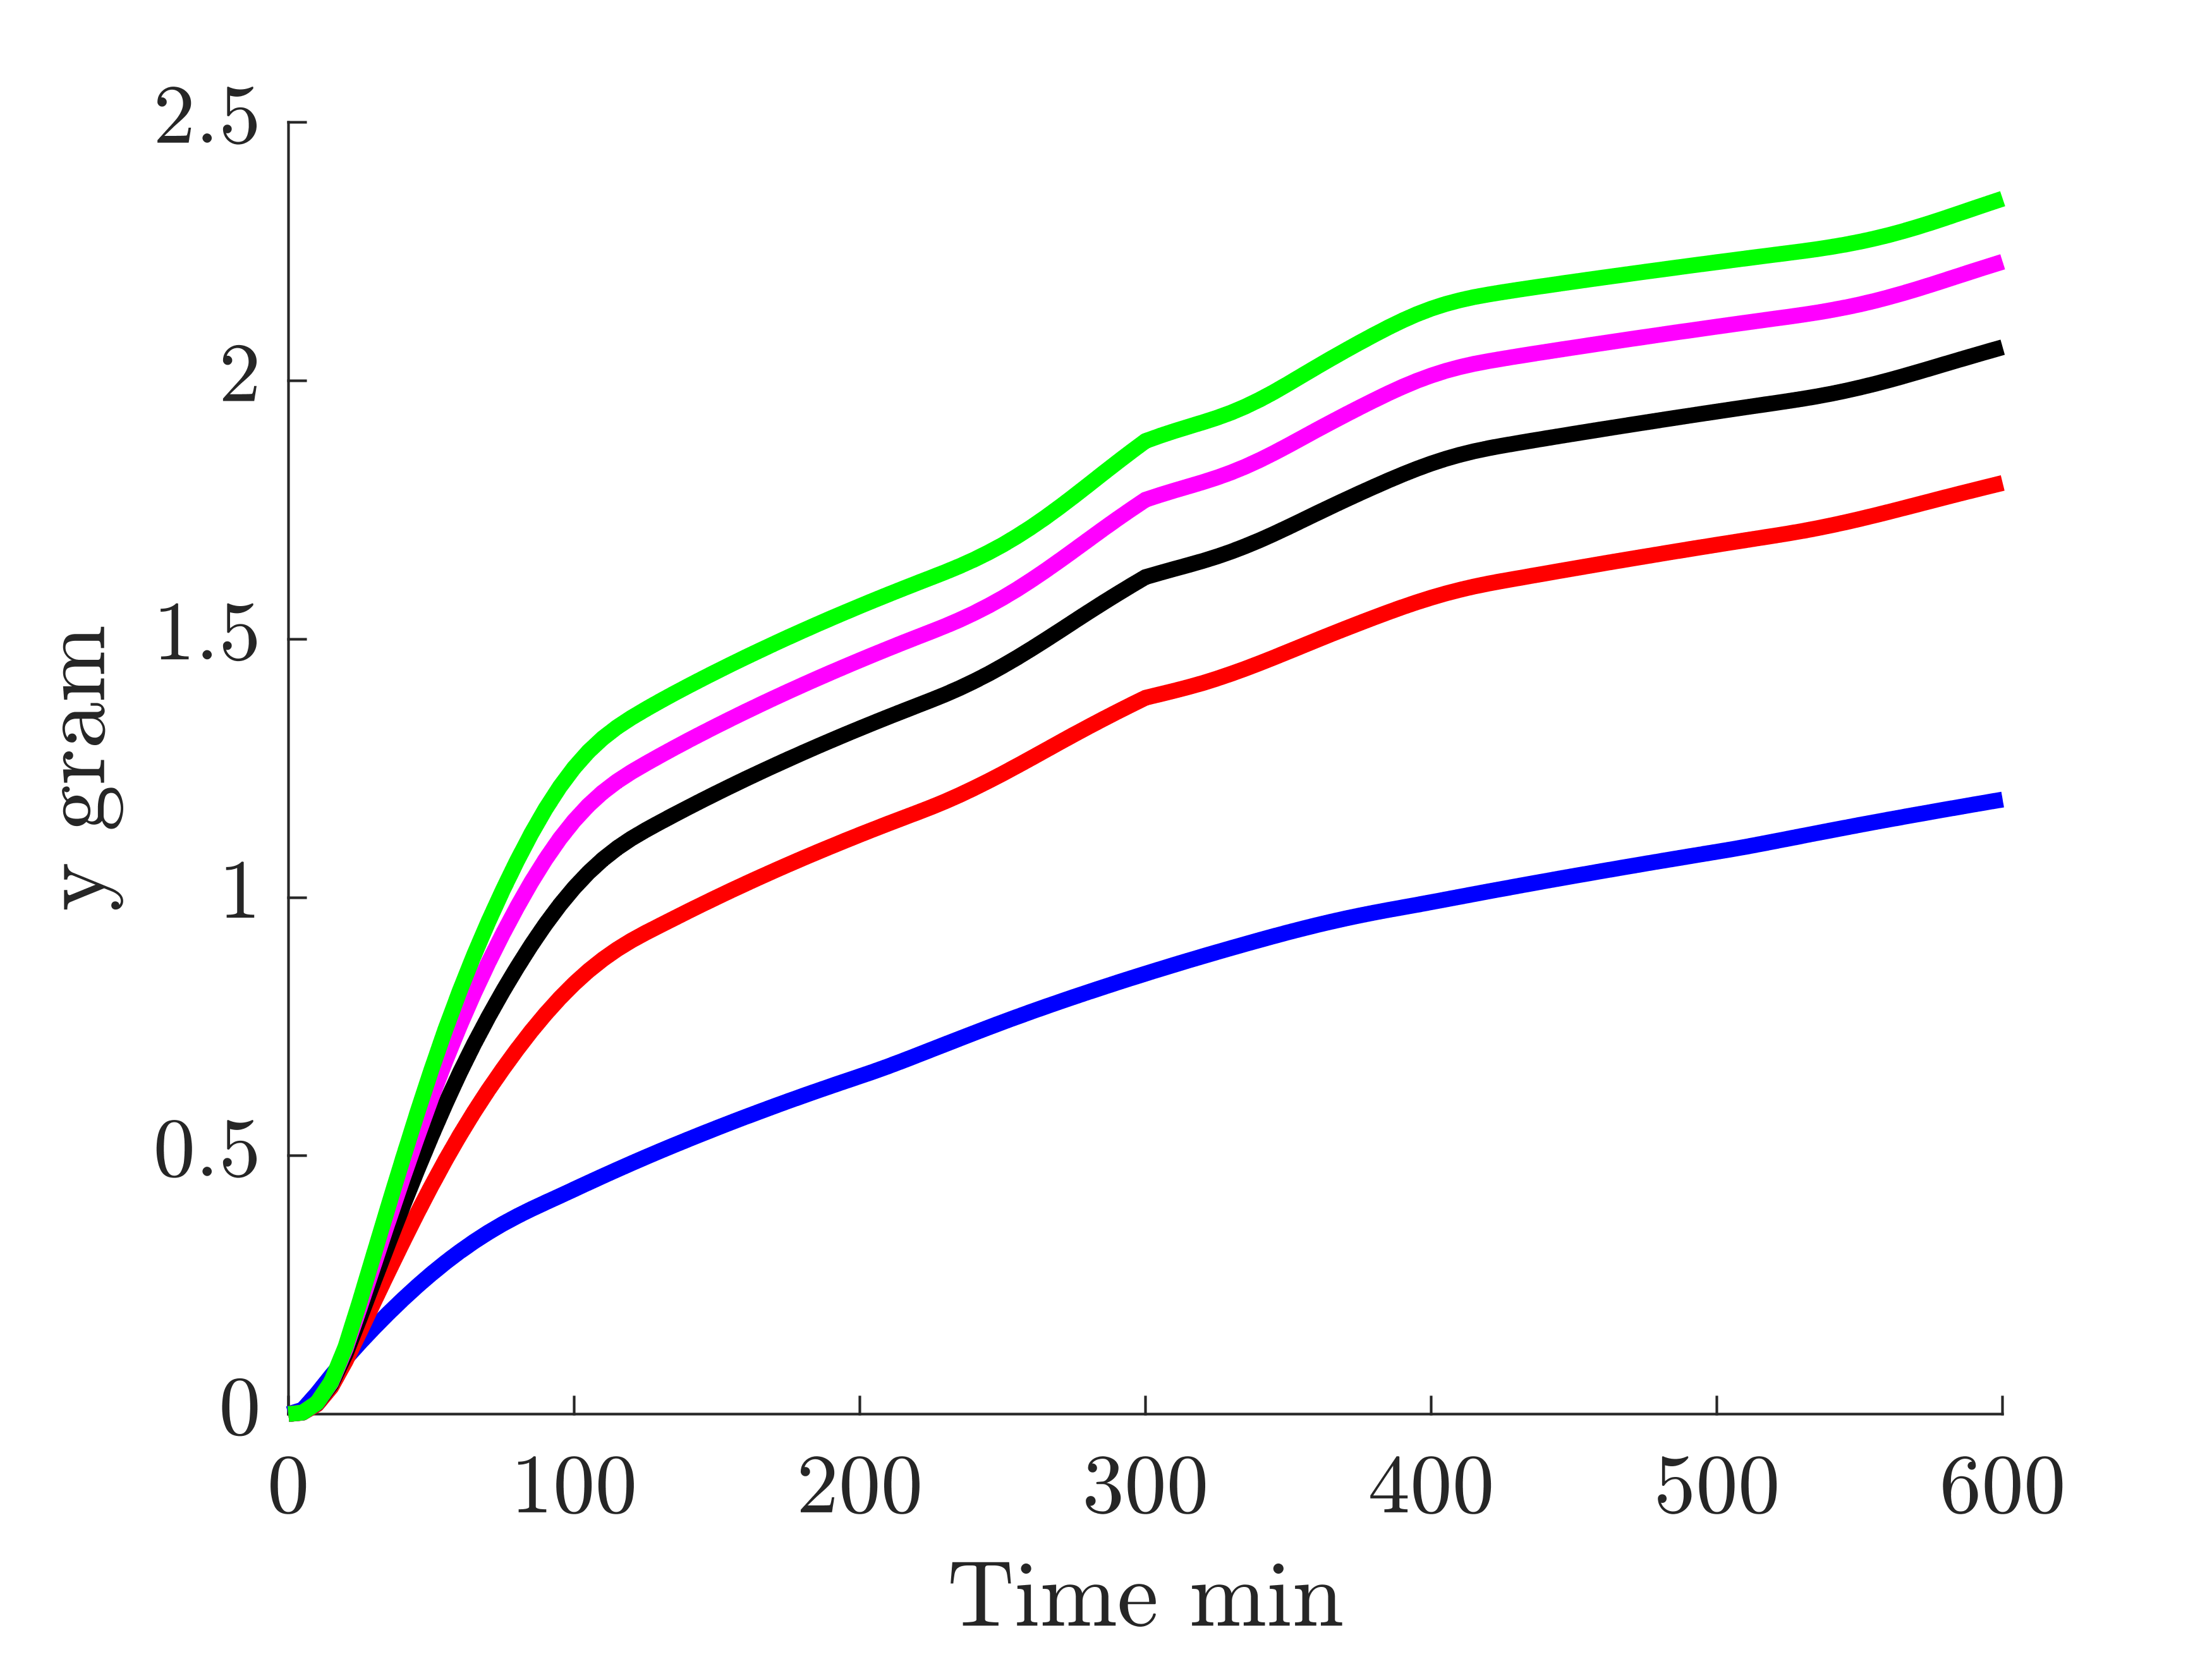
\includegraphics[width=0.90\columnwidth]{Figures/Results/yield.png}	
			\caption{Optimal yield profiles}
			\label{fig:profiles_y}
		\end{subfigure}
		\caption{Results of the optimization problem}
	\end{figure}	
	
	Figure \ref{fig:profiles_T} shows the optimal profiles of the inlet temperature ($T^{in}$) for various pressure cases in the supercritical CO$_2$ extraction process. Initially, the $T^{in}$ remains constant at approximately $40~^\circ C$ for all pressures, indicating a stable starting condition for the system. The temperature decreases after about 300 min, but the exact time slightly varies depending on the pressure. This decline is rapid for lower pressures and gradual for higher pressures. The blue curve (100 bar) exhibits the sharpest temperature drop, while the green curve (200 bar) demonstrates a slower and more gradual decline. At lower pressures, the final temperature reaches the critical temperature and remains steady until the end of the batch. In contrary, the higher pressure cases result in a less significant temperature reduction. Moreover, the system does not reach steady operating conditions, as the inlet temperature profile does not flatten by the end of the process.

	Figure \ref{fig:profiles_y} depicts the predicted yield curves. A closer examination of the yield and scatter plots reveals that the most informative experiments do not necessarily correspond to those with the highest yield. When the D-optimality criterion is applied, the aim is to maximize the determinant of the Fisher information matrix across the experimental design space. This approach identifies conditions that amplify variations in observed responses, particularly in regions with high sensitivity to parameter changes. As a result, the yield curve may display a "wavy" pattern, characterized by oscillations rather than a smooth, monotonic trend. These fluctuations arise from increased multiple critical points—local maxima, minima, or saddle points—on the response surface. By maximizing the sum of determinants of the Fisher information matrix, the experimental design prioritizes regions of high curvature, where the response changes sharply. 
	
	Alternatively, the D-optimality problem can be understood through the concept of Gaussian curvature. In this view, the experimental design shapes the parameter space of a model into a manifold with local geometry defined by the Fisher information matrix. The D-optimality condition maximizes the determinant of this matrix, which geometrically corresponds to maximizing the product of the principal curvatures of the manifold at a given point. This determinant is directly proportional to the Gaussian curvature, linking experimental design to the geometry of the parameter space. The determinant of the Fisher information matrix can be interpreted as a measure of the "volume element" on the parameter manifold, with higher values indicating regions of greater local curvature. By maximizing this determinant, the parameter manifold is locally as curved as possible, which explains the wavy behavior of the yield curves.
	
	The results and observations discussed in this article are local and should be considered valid only for the model given by \citet{Sliczniuk2024}. Although general conclusions about the curvature of the yield curve are independent of a process model, a completely different set of control profiles should be expected if the same technique is applied to a different model. Such strong dependence on a model is one of the most significant limitations of this work. Moreover, the model predicts the dataset in the region, which has not been validated during previous experiments. On one hand this leaves a room for model validation, on the other hand the obtained set of data points might differs from the predictions.
	
\end{document}








































